%\vspace{-4mm}

\section{Introduction}
\label{sxn:intro}

Given two or more Deep Neural Networks (DNNs) with  similar architectures, and trained on the same dataset, but trained with different solvers, parameters, hyper-parameters, regularization, etc., can we predict which DNN will have the best test accuracy, and can we do so without peeking at the test data?   

Solving this question of generalization would have both theoretical impact and great practical importance. 
With respect to the former, solving this would help to understand why this class of machine learning (ML) models performs as well as it does in certain classes of applications.
With respect to the latter, here are several motivating examples.
\begin{itemize}
\item
\textbf{Automating architecture choice.}
XXX.  AUTOMATE ARCHITECTURE CHOICE AND NOT BE TOO BRITTLE.
There is interest in automating the design of DNN models

\item
\textbf{Pre-training on smaller data.}
XXX.  KNOW HOW EO EXTRAPOLATE SMALL RESULTS FROM SMALLER DATA, WITH OUT LOTS OF BRITTLE CROSS VALIDATION.
\item
\textbf{XXX SOMETHING ELSE.}
XXX.  WHAT.  MAYBE PRACTICAL THEORY HERE, ALTHOUGH IT WOULD BE GOOD TO HAVE A REAL PROBLEM.
\end{itemize}

To address our main question, we will build upon and combine two seemingly-unrelated lines of recent work.
The first is the recent work of Martin and Mahoney~\cite{MM17_TR,MM18_TR}, who used Statistical Mechanics (SM) methods and Heavy-Tailed (HT) Random Matrix Theory (RMT) to analyze the weight matrices of DNNs, including both (large) production-quality pre-trained models as wel as (small) models trained from scratch.
The second is a large body of work~\cite{XXX-XXX,XXX-XXX,XXX-XXX,XXX-XXX}, perhaps the most recent and related of which is that of Liao et al.~\cite{LMBx18_TR}, who use norm-based capacity control metrics to bound generalization error.

The recent work of Martin and Mahoney~\cite{MM18_TR} used the the Universality underlying HT-RMT to characterize the Implicit Self-Regularization in well-trained DNNs.
Among other things, they showed that the empirical spectral density (ESD) of DNN layer matrices for nearly every large state-of-the-art pre-trained production-quality DNN displays HT behavior, e.g., that it is well-fit by a power law (PL) distribtion.
%
The original work~\cite{MM18_TR} considered 
NNs including AlexNet and InceptionV3 (as well as DenseNet, ResNet, and VGG),
and subsequent work~\cite{MM18_unpub_work} has shown that these results are ubiquitous. 
Upon examining nearly 10,000 layer weight matrices $\mathbf{W}_{l,i}$ across over 50 different modern pre-trained DNN architectures, the ESD of nearly every $\mathbf{W}$ layer matrix can be fit to a PL:
$70-80\%$ of the time, the fitted PL exponent $\alpha$ lies in the range $\alpha\in(2,4)$ (in the Moderately Heavy-Tailed Universality class); and
$10-20\%$ of the time, the fitted PL exponent $\alpha$ lies in the range $\alpha< 2$ (in the Very Heavy-Tailed Universality class).
Of course, there are exceptions: in any real DNN, the fitted $\alpha$ may range anywhere from $\sim 1.5$ to $10$ or higher~\cite{MM18_unpub_work}.  

In the SM analysis of complicated systems, e.g., well-trained NNs~\cite{EB01_BOOK,nishimori01}, this kind of Universality of PL exponents is very special and suggests the presence of a deeper, underlying mechanism driving the system~\cite{SornetteBook,BouchaudPotters03}. 
Perhaps the most well-known form of Universality is associated with the Gaussian Universality class, where it is known that the sum of many random variables drawn from a wide range of distributions are ``approximately Gaussian,'' e.g., in the sense that it approaches a suitably-normalized Gaussian distribution.
As briefly reviewed below, and ad described in more detail in~\cite{MM18_TR} HT Universality makes analogous (but, admittedly, more complicated) statements for random variables drawn from distributions in which the tails decay more slowly than those in the Gaussian Universality class~\cite{XXX-XXX,XXX-XXX}.
It is this Universality that originally motivated this study.

XXX.  PAR ON THE MOTIVATION AND DERIVATION OF OUR WEIGHTED PL ESTIMATOR.
This suggests that we look for a Universal capacity metric, i.e., one that XXX SUCH AND SUCH.
A natural candidate for this is the sum of PL exponents.
For $\alpha \gtrsim 1$, we show XXX, which---due to Universality---we assume holds for a broader range of $\alpha$.
XXX.  FIX.

Our main results consist in performing a detailed empirical evaluation of this Universal capacity control metric, illustrating that it works, in the sense that XXX SUCH AND SUCH.
That it works over a much broader range than our original derivation permits is presumably due to the underlying Universality.
XXX.  FIX.

We also consider the approximation to our Universal capacity control metric that is simply the average log Frobenius norm of the layers.
This is quicker to compute, and which we show works, XXX BUT NOT AS WELL.
Interestingly, this approximation is related to the recent results of Liao et al.~\cite{LMBx18_TR}, who build on recent work \cite{SHNx17_TR,PLMx18_TR}.
XXX.  FIX.


This line of norm-based capacity control metrics work has been motivated by the observation that parameter counting and more traditional VC-based bounds tend to lead to vacuous results for modern state-of-the-art DNNs.
There are many reasons for this (see, e.g., the discussion in~\cite{MM17_TR,MM18_TR}, but an important one is that modern DNNs are heavily over-parameterized.
The most related recent work is that of \cite{LMBx18_TR}, who XXX WORKED ON SMALL DATA OR WHATEVER, DESCRIBE WHAT THEY DID, AND BE EXPLICIT ABOUT NORMALIZATION/SCALING ISSUES.
XXX.  FIX.

Indeed, our main results can approximated by the weighted Product Norm of Liao et al.~\cite{LMBx18_TR} (as we show XXX WHERE), extended and refined to take into account the heavy-tailed and finite-size issues highlighted by the recent HT-RMT-based analysis of Martin and Mahoney~\cite{MM18_TR}.
XXX.  FIX.

(((
\charlesX{
We apply our new Theory of Heavy-Tailed Self Regularization (HT-SR) to analyze these large, pre-trained DNNs.  
We model \emph{the correlations} arising in the DNN layers by forming the normalized correlation matrices $\mathbf{X}=(1/N)\mathbf{W}_{L}^{T}\mathbf{W}_{L}$ 
for each of the individual  the layer weight matrices $\mathbf{W}_{L}$ and then studying the eigenvalue density of each $\mathbf{X}$,  $\rho(\lambda)$.
The HT-SR Theory lets us characterize the densities because they almost always display heavy tailed signatures,
 and can be fit to a Power Law, $\rho(\lambda)\sim\lambda^{-\alpha}$, with exponent $\alpha$.   And , on average,
 the smaller the $\alpha$, the more Self Regularization is in the DNN.  Of course, the
  pre-trained weight matrices  $\mathbf{W}_{L}$  themselves are not at all random because they have been trained 
  on very large, high quality data sets,
  and they behave quite differently from a random heavy tailed (i.e. Pareto) matrix.  And it is these differences we can exploit
  to predict trends in the generalization accuracy.}
\michael{Where exactly to put this.}
)))
  


As an example of our main results, consider Figure~\ref{fig:vgg}, which shows both the average log Frobenius norm 
($\langle\log\Vert\mathbf{W}\Vert_{F}\rangle$, defined in Eqn.~(\ref{eqn:av_log_norm}))
as well as the weighted average PL exponent ($\hat{\alpha}$, defined in Eqn.~(\ref{eqn:alpha_hat_specific}))
as a function of the reported (Top1) test accuracy for the series of pre-trained VGG models (available in the pyTorch package~\cite{pyTorch}).
(See Table~\ref{table:models_VGG} for additional details.)
Figure~\ref{fig:vgg_lognorms} shows the average log Frobenius norm results, which are quite good; and 
Figure \ref{fig:vgg_alphahat} shows the weighted average PL exponent results, which yield slight improvements due to the method we introduce.
Importantly, since we are using reported test accuracies (i.e., from the literature, and not due to the pecularities of our training), we did not need to retrain any models.
Equally importantly, we did not need to peek at the ImageNet test data to make this plot; and, in fact, we did not even need the ImageNet training data either.  


\begin{figure}[t] %[!htb]
   \centering
   \subfigure[log Frobenius norm $\langle\log\Vert\mathbf{W}\Vert_{F}\rangle$]{
      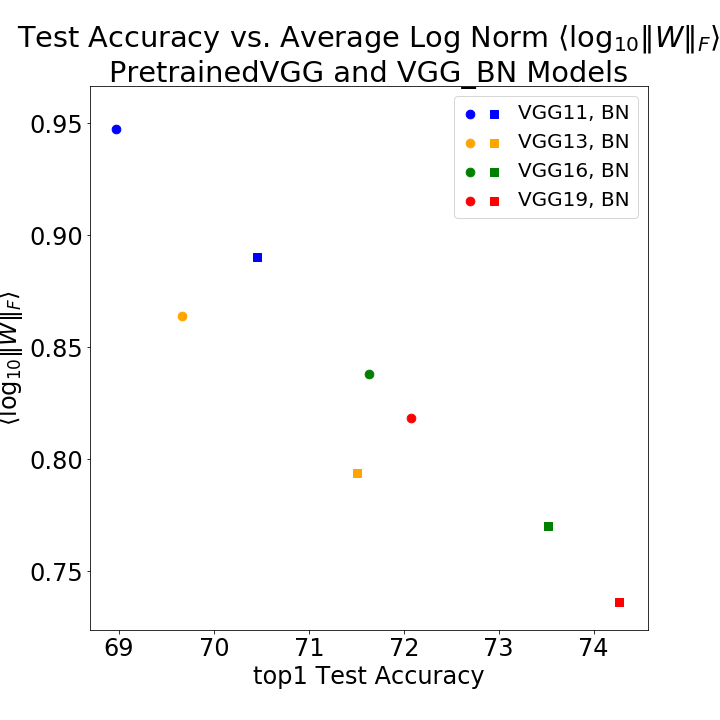
\includegraphics[scale=0.35]{img/vgg-lognorms.png}
      \label{fig:vgg_lognorms}
   }
   \subfigure[weighted average PL exponent $\hat{\alpha}$]{
      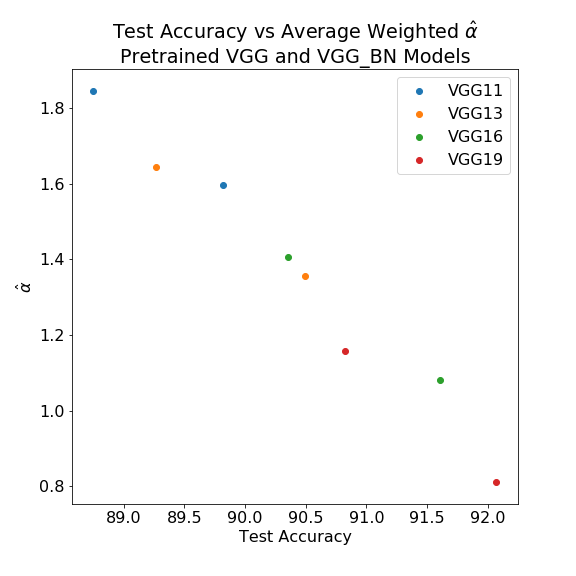
\includegraphics[scale=0.35]{img/vgg-w_alphas.png}
      \label{fig:vgg_alphahat}
   }
   \caption{%
      Pre-trained VGG and VGG\_BN Architectures and DNNs.  
      Test Accuracy versus
      average log Frobenius norm $\langle\log\Vert\mathbf{W}\Vert_{F}\rangle$ (in (\ref{fig:vgg_lognorms}))
      or
      weighted average PL exponent $\hat{\alpha}$ (in (\ref{fig:vgg_alphahat}))
      for
      VGG11 vs VGG11\_BN ({\color{blue}{blue}}),
      VGG13 vs VGG13\_BN ({\color{orange}{orange}}),
      VGG16 vs VGG16\_BN ({\color{green}{green}}),  and
      VGG19 vs VGG19\_BN ({\color{red}{red}}). 
      \michael{Have circles and squares or something like that to distinguish regular and BN versions.}
   }
   \label{fig:vgg}
\end{figure}


%% COMBINED WITH ABOVE %% \begin{figure}[!htb]
%% COMBINED WITH ABOVE %%  \centering
%% COMBINED WITH ABOVE %%    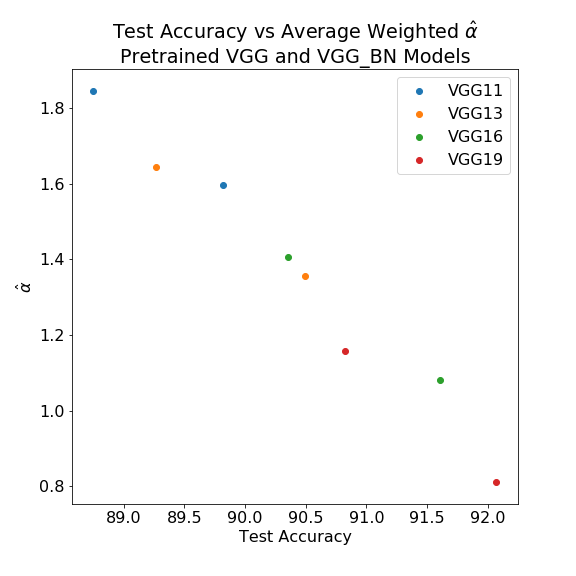
\includegraphics[scale=0.40]{img/vgg-w_alphas.png}
%% COMBINED WITH ABOVE %%    \caption{
%% COMBINED WITH ABOVE %% Pre-trained VGG and VGG BN Architectures and DNNs.  Test Accuracy and weighted average $\hat{\alpha}$ for
%% COMBINED WITH ABOVE %%  VGG11 vs VGG11\_BN ({\color{blue}{blue}}),
%% COMBINED WITH ABOVE %% VGG13 vs VGG13\_BN ({\color{orange}{orange}}),
%% COMBINED WITH ABOVE %% VGG16 vs VGG16\_BN ({\color{green}{green}}),  and
%% COMBINED WITH ABOVE %% VGG19 vs VGG19\_BN ({\color{red}{red}}). 
%% COMBINED WITH ABOVE %% }
%% COMBINED WITH ABOVE %%   \label{fig:vgg_alphahat}
%% COMBINED WITH ABOVE %% \end{figure}


In summary, our main results are the following:
\begin{itemize}
\item
We apply the Product Norm regularization metric to a wide range of production-level DNN models, including the VGG and ResNet series of models, illustrating that it performs quite well.
To our knowledge, this is the first time this theoretical capacity metric has been reported to predict (trends in) the test accuracy for \emph{pre-trained production-level} DNNs, illustrating the usefulness of these norm-based metrics beyond smaller models such as MNIST, CIFAR10, and CIFAR100. 
%%This in itself is remarkable. 
%%But we can do even better than this -- by exploiting Heavy Tail Universality.
\item
We use HT-RMT, and in particular the Universality properties of the recently-developed theory of Implicit Self-Regularization to develop a novel capacity metric based on the HT structure of these models.
%%\charlesX{THIS:  We use our recently-developed Theory of Heavy Tailed Self-Regularization (HT-SR) to develop a novel capacity metric}
This metric is a weighted linear combination of PL exponents, where the coefficients are the \emph{Spectral} norm of the associated weight matrices.
This metric may be viewed as a refinement of the \emph{Frobenius} norm Product Norm metric that accounts for the HT and finite-size effects.
\item
We apply this novel metric to the VGG and ResNet series of models, comparing it with the Product Norm metric.
In general, it does comparable to or slightly better than the Frobenius norm metric.
We also apply it to a wide range of other pre-trained DNN models, including XXX, XXX, and XXX.
\michael{Ques: which exactly make the final cut to be~included.}
\end{itemize}

We conclude this introduction with two higher-level comments.
%
First, 
one of the main insights of our approach is to highlight the importance of what might seem to be a technical issue to ignore, but which in our experience is \emph{extremely} important: the scaling or normalization for weight matrices used in the DNN, and how this relates to the difference between finite-sized versus asymptotic effects.
This scaling issue has been highlighted perhaps most recently by Liao et al.~\cite{LMBx18_TR}, who were interested in showing that classical generalization bounds can be tight, when normalization is performed appropriately.
Our approach complements this; and, to our knowledge, our approach is the first to highlight the connection with finite-size effects.
%
Second, 
%it is worth emphasizing that 
we are taking a 
very %somewhat 
non-standard approach (at least for the DNN and ML communities) to address our main question.
We won't train/retrain lots and lots of (typically rather small) models, analyzing training/test curves, trying to glean from them bits of insight that might then extrapolate to more realistic models.
Instead, we will take advantage of the fact that there already exist many (typically rather large) publicly-available pre-trained models, and we will analyze the properties of these models.
That is, we will view these publicly-available pre-trained models as artifacts of the world that achieve state-of-the-art performance in computer vision (CV), natural language processing (NLP), and related applications; and we will attempt to understand why.
To do so, we will analyze the empirical (spectral) properties of these models; 
%from this, we will form a hypothesis as to why they perform well; 
and we will then extract data-dependent metrics to predict their generalization performance on production-quality models.
Given well-known challenges associated with training, and given our results here as well as other recent results~\cite{MM18_TR}, we suggest that this methodology be applied more generally.

